\documentclass[11pt]{article}
\usepackage{fancyhdr, extramarks, amsmath, amsthm, amsfonts, tikz, algpseudocode, graphicx, tcolorbox}
\usepackage[plain]{algorithm}
\graphicspath {{graphs/}}
\usetikzlibrary{automata,positioning}
\usepackage{geometry}\geometry{letterpaper,
  	left=0.75in, right=0.75in,
  	top=1in, bottom=1in,
  	headsep=.2in }
\title{\textbf{Introduction to Artificial Intelligence\\
		\large Project 4: Colorization}}
\author{Brenton Bongcaron and Abe Vitangcol\\NetIDs: bdb101 and alv88}
\date{May 5, 2021}
\begin{document}
	\maketitle
\textit{We have read and abided by the rules laid out in Canvas, We have not used anyone else's work for our project, and our work is only our own.}
\tableofcontents
\listoffigures
\pagebreak
\section{Introduction}

Imagine this: you want to send an image to someone, but trying to send the image will cause some error, saying how the image was too large to send. This is commonly seen on applications such as Discord where they limit the size of the images people are allowed to send (unless, with paid perks of course) and the image cannot send. So, instead, the image gets rejected to send unless it has been compressed to lower the size of the image file. So, then the question becomes: how does the image become compressed and the file size becomes lower than the original? The answer: through simplifying the image into similar colors, thus reducing the size. Hence, this project will do such thing, simplifying an image and use less colors to represent the same thing.

\section{The Image}
To test out our algorithms to see how well it does, we have to use a common image and see the algorithm's quality in terms of both representation (how well it represents the original image) and in terms of aesthetics (how appealing it looks to the eye). The image needs to have a balance of colors on both sides and not too much of a color spread. The image we needed was, in fact, the doge, and thus, the doge became the image we tested on.

\begin{figure}[h]
\centering
\includegraphics[scale=1.10]{images/smoldoge.jpg}
\caption{Wow, such beauty, much colors, many fun. Will it go to the moon?}
\end{figure}

\section{The Basic Agent}
To start, the basic agent was necessary as a baseline of how well our advanced algorithm works. The basic agent begins with clustering the colors into 5 best representative colors using k-Nearest Neighbors calculations. Then, the basic agent has 2 arrays, one a grayscale verison of the doge, the other the original image. Using the left half of the grayscale image as training, it replaces 3x3 patches with one of the representative colors accordingly. Then it goes to the right half and tries to fill in the rest of the colors based on what it learned through the training, with a black border around the right half because of how some tiles do not give enough information to complete the image. The result is shown in Figure 2.

\begin{figure}[h]
\begin{minipage}[c]{0.5\textwidth}
\centering
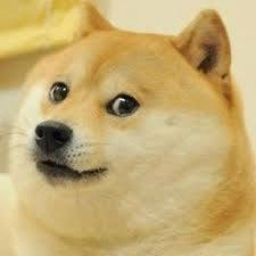
\includegraphics[scale=0.94]{images/smolDoge.jpg}
\begin{center}
Original
\end{center}
\end{minipage}
\begin{minipage}[c]{0.5\textwidth}
\centering
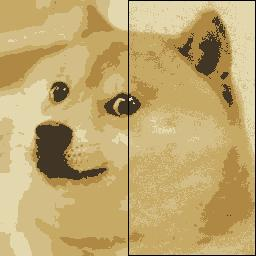
\includegraphics[scale=0.70]{images/basic.jpg}
\begin{center}
Basic Agent
\end{center}
\end{minipage}
\caption{Colors Much, Beauty Such, Woah.}
\end{figure}
\section{The Advanced Agent}
\subsection{The Math}
First, we define the sigmoid function:
\[
g(z) = \frac{1}{1+e^{-z}}
\]
\[
g'(z) = g(z)(1-g(z))
\]
The model that we build for each color returns a value from 0 to 1, which is the normalized R or G or B value that a pixel will be colored with:
\[
f_{\underline{wY}}(\underline{x}) = \frac{1}{1 - e^{-(\underline{wY}. \underline{x})}} = \frac{1}{1 - e^{-(Y(\underline{x}))}} = g[Y(\underline{x})]
\]
where:
\begin{itemize}
\item $\underline{wY}$ is the weights for the weight vector corresponding to the model for color $Y \in \{R, G, B\}$
\item $\underline{x}$ is the vector containing the \textit{normalized }grayscale values of the grayscale patch corresponding to the pixel to be colored (the real grayscale value is $255\cdot x_j$)
\item $f_{\underline{wY}}(\underline{x})$ returns a \textit{normalized} value of a color (the real value of the color is $255\cdot f_{\underline{w}}(\underline{x})$)
\end{itemize}
We defined our loss function to be a sum of the square error between :
\[
\text{Loss}(f_{\underline{w}}(\underline{x}),y) = [\text{y} - 255\cdot f_{\underline{wY}}(\underline{x})]^2 = [\text{y} - 255\cdot g(Y(\underline{x}))]^2
\]
where $y$ is the actual value for the color $y \in \{r, g, b\}$ in the original image's matrix.\\\\
Using the chain rule to start calculating the gradient of the loss function:
\[
\frac{\partial}{\partial wY_j}\text{Loss}(f_{\underline{w}}(\underline{x}),y) = \frac{\partial}{\partial wY_j}\left[\text{y} - 255\cdot g(Y(\underline{x}))\right]^2
\]
\[
= 2\cdot[y - 255\cdot g(Y(\underline{x}))]\cdot\frac{\partial}{\partial wY_j}[\text{y} - 255g(Y(\underline{x}))]
\]
\[
= 2\cdot\left[y - 255\cdot g(Y(\underline{x}))\right]\cdot\frac{\partial}{\partial wY_j}[-255\cdot g(Y(\underline{x}))] 
\]
\[
=  2\cdot[y - 255\cdot g(Y(\underline{x}))]\cdot[-255\cdot g'(Y(\underline{x}))]\cdot\frac{\partial}{\partial wY_j}[Y(\underline{x})]
\]
Note that by construction of our definition of our model:
\[
Y(\underline{x}) = \underline{wY}.\underline{x} = wY_0\cdot x_0 + wY_1\cdot x_1 + wY_2\cdot x_2 + wY_3\cdot x_3 + wY_4\cdot x_4 + wY_5\cdot x_5 + wY_6\cdot x_6 + wY_7\cdot x_7 + wY_8\cdot x_8 + wY_9\cdot x_9
\]
Similar to how it was done in lecture, we define $x_0 = 1$, but we left it in explicit terms of the dot product for smooth notation. Thus:
\[
\frac{\partial}{\partial wY_j}[Y(\underline{x})] = x_j
\]
where $x_j$ is the $j^{th}$ component of the grayscale vector.\\\\
Continuing the calculation of the gradient of the loss function:
\[
\frac{\partial}{\partial wY_j}\text{Loss}(f_{\underline{w}}(\underline{x}),y) =  2\cdot[y - 255\cdot g(Y(\underline{x}))]\cdot[-255\cdot g(Y(\underline{x}))]\cdot\frac{\partial}{\partial wY_j}[Y(\underline{x})]
\]
\[
=  2\cdot[y - 255\cdot g(Y(\underline{x}))]\cdot[-255\cdot g'(Y(\underline{x}))]\cdot x_j
\]
Plugging in the definition of the derivative of the sigmoid function:
\[
=  2\cdot[y - 255\cdot g(Y(\underline{x}))]\cdot -255\cdot g(Y(\underline{x}))\cdot(1 - g(Y(\underline{x})))\cdot x_j
\]
\[
=  -2\cdot[y - 255\cdot g(Y(\underline{x}))]\cdot [255\cdot g(Y(\underline{x}))]\cdot(1 - g(Y(\underline{x})))\cdot x_j
\]
\[
=  2\cdot[255\cdot g(Y(\underline{x}))-y]\cdot [255\cdot g(Y(\underline{x}))]\cdot(1-g(Y(\underline{x})))\cdot x_j
\]
Thus:
\[
\nabla\text{Loss}_{wY_j}(f_{\underline{w}}(\underline{x}),y) =  2\cdot[255\cdot g(Y(\underline{x}))-y]\cdot [255\cdot g(Y(\underline{x}))]\cdot(1-g(Y(\underline{x})))\cdot \underline{x}
\]
Using Stochastic Gradient Descent, we now have a formula to update the weights of our color models:
\[
\underline{wY}(k+1) = \underline{wY}(k) - \alpha\nabla\text{Loss}_{wY_j}(f_{\underline{w}}(\underline{x}),y)
\]
\[
= \underline{wY}(k) - \alpha\cdot 2\cdot[255\cdot g(Y(\underline{x}))-y]\cdot [255\cdot g(Y(\underline{x}))]\cdot(1-g(Y(\underline{x})))\cdot \underline{x}
\]
\[
= \underline{wY}(k) - \alpha\cdot[255\cdot g(Y(\underline{x}))-y]\cdot [255\cdot g(Y(\underline{x}))]\cdot(1-g(Y(\underline{x})))\cdot \underline{x}
\]
Note that the constant $2$ in the gradient of the loss function was absorbed into the learning rate constant.\\\\
In terms of English words, the formula to update the weights of our color models can be written as:
\[
\text{New weights} = (\text{old weights}) - (\text{learning rate})(\text{predicted}-\text{actual})(\text{predicted})(1-\frac{\text{predicted}}{255})(\text{grayscale vector})
\]
where "weights" implies the weight vector of a color model.
\subsection{The Code}
The following function is pseudo-code for our training algorithm for each of our color models and is located in \verb|train.py|.
\begin{verbatim}
def weightFitting(image):
    im_width, im_height <- image.size
    rgbMatrix <- numpy matrix form of image
    grayIm <- numpy matrix form of grayscale image
    alpha = 0.0001
    wR <- initialization of all weights for "red" model to 0.5
    wG <- initialization of all weights for "blue" model to 0.5
    wB <- initialization of all weights for "green" model to 0.5
    for 150000 rounds of training:
        randPixel <- random pixel on LEFT side of image
        r, g, b <- RGB values of randPixel
        gray = [1]
        for x in range(-1,2):
             for y in range(-1,2):
                  currentPixel <- (randPixel[0]+x, randPixel[1]+y) 
                  gray.append(grayscale value, divded by 255, of currentPixel)
                  
        # Note that dotP() means dot product
        Rx = dotP(wR, gray)
        Gx = dotP(wG, gray)
        Bx = dotP(wB, gray)

        predR = 255.0 / (1 + exp(-1 * Rx))
        predG = 255.0 / (1 + exp(-1 * Gx))
        predB = 255.0 / (1 + exp(-1 * Bx))

        gLossR = [(predR - r)*predR*(1 - predR/255.0)*gray[i] for i in range(len(gray))]
        gLossG = [(predG - g)*predG*(1 - predG/255.0)*gray[i] for i in range(len(gray))]
        gLossB = [(predB - b)*predB*(1 - predB/255.0)*gray[i] for i in range(len(gray))]

        update the weights of the colors' models
        
    return the weights of the colors' models
\end{verbatim}

This is what is used to update and return the weights of the colors after all the trials. Note $\alpha$ and the initial weight values seen within the code were found by performing many tests and checking various values before settling on the current values seen. As for the training, more was better since the weights was going converge anyway, meaning it will avoid overfitting, and the training was fast, so more was done for more consistent colors per test. This concludes the function weightFitting, with the weights of the colors returned to the advanced agent, where it uses them to complete the picture.

For our function, the input space is a grayscale patch in the form of a vector and the output space is the RGB values of the center pixel the function is observing within the grayscale patch. None of the input data, other than the conversions of pixels to grayscale, has been preprocessed or processed outside of the function before being inputted.

\pagebreak
\subsection{The Results}
The result of the Advanced AI is shown in Figure 3.

\begin{figure}[h]
\begin{minipage}[c]{0.5\textwidth}
\centering
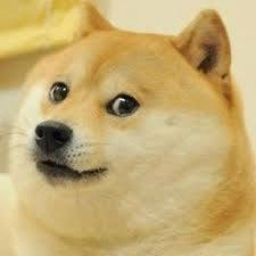
\includegraphics[scale=0.94]{images/smolDoge.jpg}
\begin{center}
Original
\end{center}
\end{minipage}
\begin{minipage}[c]{0.5\textwidth}
\centering
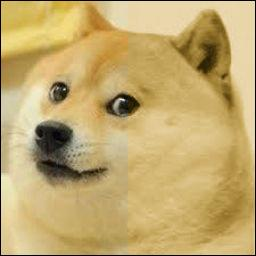
\includegraphics[scale=0.70]{images/advanced.jpg}
\begin{center}
Advanced Agent
\end{center}
\end{minipage}
\caption{Wow, such beauty, much shading, many wows.}
\end{figure}

In terms of quality, it definitely has more colors than the basic agent and, aesthetically speaking, it looks much better than the, err... abstract art doge. The advanced agent colors and shades the doge really well and, in terms of time, completes the doge faster than the basic agent. The basic agent takes around 7 minutes to complete its picture whereas the advanced agent took only 30 seconds to a minute to complete with a better quality. Given how both used the same picture and the way both agents completed the doge, it seemed fair to say the basic agent was not as capable as the advanced agent, but both did their jobs well. With how well the advanced agent does, it was given the name \textbf{Stronk Vectoral Weightroom}, or \textbf{SVW}.

However, should there be enough time and resources to complete this (and not a span of two to three weeks because of unfortunate college classes), there would be plans to use neural networks to color the image. There would also be plans to make the algorithm faster (faster than 30 seconds because there is never anything wrong with faster) and test it on more than just doge.

\section{Contributions}
\subsection*{Brenton Bongcaron [bdb101], Section 3}
I did all of the coding of the basic and advanced agents. I also made edits to the \LaTeX\: document.
\subsection*{Abe Vitangcol [alv88], Section 8}
I completed this \LaTeX\: document and did some proofreading and commenting on the code. Wording the \LaTeX\: document was something both my partner and I agreed I liked doing as well as having fun with the doge memes here. Unfortunately, many things came up on my end (mainly affecting my mental health) and thus I wasn't able to work on this project as much as I wanted to. Many apologies to my partner for being unable to help well on this one.
\end{document}